% This file is generated by the MATLAB m-file laprint.m. It can be included
% into LaTeX documents using the packages graphicx, color and psfrag.
% It is accompanied by a postscript file. A sample LaTeX file is:
%    \documentclass{article}\usepackage{graphicx,color,psfrag}
%    \begin{document}% This file is generated by the MATLAB m-file laprint.m. It can be included
% into LaTeX documents using the packages graphicx, color and psfrag.
% It is accompanied by a postscript file. A sample LaTeX file is:
%    \documentclass{article}\usepackage{graphicx,color,psfrag}
%    \begin{document}% This file is generated by the MATLAB m-file laprint.m. It can be included
% into LaTeX documents using the packages graphicx, color and psfrag.
% It is accompanied by a postscript file. A sample LaTeX file is:
%    \documentclass{article}\usepackage{graphicx,color,psfrag}
%    \begin{document}% This file is generated by the MATLAB m-file laprint.m. It can be included
% into LaTeX documents using the packages graphicx, color and psfrag.
% It is accompanied by a postscript file. A sample LaTeX file is:
%    \documentclass{article}\usepackage{graphicx,color,psfrag}
%    \begin{document}\input{f_Qs_30_p_5_2}\end{document}
% See http://www.mathworks.de/matlabcentral/fileexchange/loadFile.do?objectId=4638
% for recent versions of laprint.m.
%
% created by:           LaPrint version 3.16 (13.9.2004)
% created on:           12-Nov-2008 21:50:28
% eps bounding box:     17.5 cm x 13.125 cm
% comment:              
%
\begin{psfrags}%
\psfragscanon%
%
% text strings:
\psfrag{s05}[b][b]{{\tiny $\xi_{5}$}}%
\psfrag{s06}[b][b]{{\tiny $\xi_{25}$}}%
\psfrag{s07}[b][b]{{\tiny $\xi_{35}$}}%
\psfrag{s08}[t][t]{{\tiny $\nu$}}%
\psfrag{s09}[b][b]{{\tiny $\xi_{\nu}$}}%
\psfrag{s10}[t][t]{{\tiny Slot number}}%
\psfrag{s11}[b][b]{{\tiny $F_{slot}/\SI{}{A}$}}%
%
% xticklabels:
\psfrag{x01}[t][t]{{\tiny 0}}%
\psfrag{x02}[t][t]{{\tiny 5}}%
\psfrag{x03}[t][t]{{\tiny 10}}%
\psfrag{x04}[t][t]{{\tiny 15}}%
\psfrag{x05}[t][t]{{\tiny 20}}%
\psfrag{x06}[t][t]{{\tiny 25}}%
\psfrag{x07}[t][t]{{\tiny 30}}%
\psfrag{x08}[t][t]{{\tiny 0}}%
\psfrag{x09}[t][t]{{\tiny 10}}%
\psfrag{x10}[t][t]{{\tiny 20}}%
\psfrag{x11}[t][t]{{\tiny 30}}%
\psfrag{x12}[t][t]{{\tiny 40}}%
\psfrag{x13}[t][t]{{\tiny 50}}%
\psfrag{x14}[t][t]{{\tiny 60}}%
%
% yticklabels:
\psfrag{v01}[r][r]{{\tiny -2}}%
\psfrag{v02}[r][r]{{\tiny -1}}%
\psfrag{v03}[r][r]{{\tiny 0}}%
\psfrag{v04}[r][r]{{\tiny 1}}%
\psfrag{v05}[r][r]{{\tiny 2}}%
\psfrag{v06}[r][r]{{\tiny 0}}%
\psfrag{v07}[r][r]{{\tiny 0.1}}%
\psfrag{v08}[r][r]{{\tiny 0.2}}%
\psfrag{v09}[r][r]{{\tiny 0.3}}%
\psfrag{v10}[r][r]{{\tiny 0.4}}%
\psfrag{v11}[r][r]{{\tiny 0.5}}%
\psfrag{v12}[r][r]{{\tiny 0.6}}%
\psfrag{v13}[r][r]{{\tiny 0.7}}%
\psfrag{v14}[r][r]{{\tiny 0.8}}%
\psfrag{v15}[r][r]{{\tiny 0.9}}%
\psfrag{v16}[r][r]{{\tiny 1}}%
\psfrag{v17}[r][r]{{\tiny 1.1}}%
%
% Figure:

\subfloat[Slot mmf and winding factors\label{fig:f_Qs30_p5_2}]{%
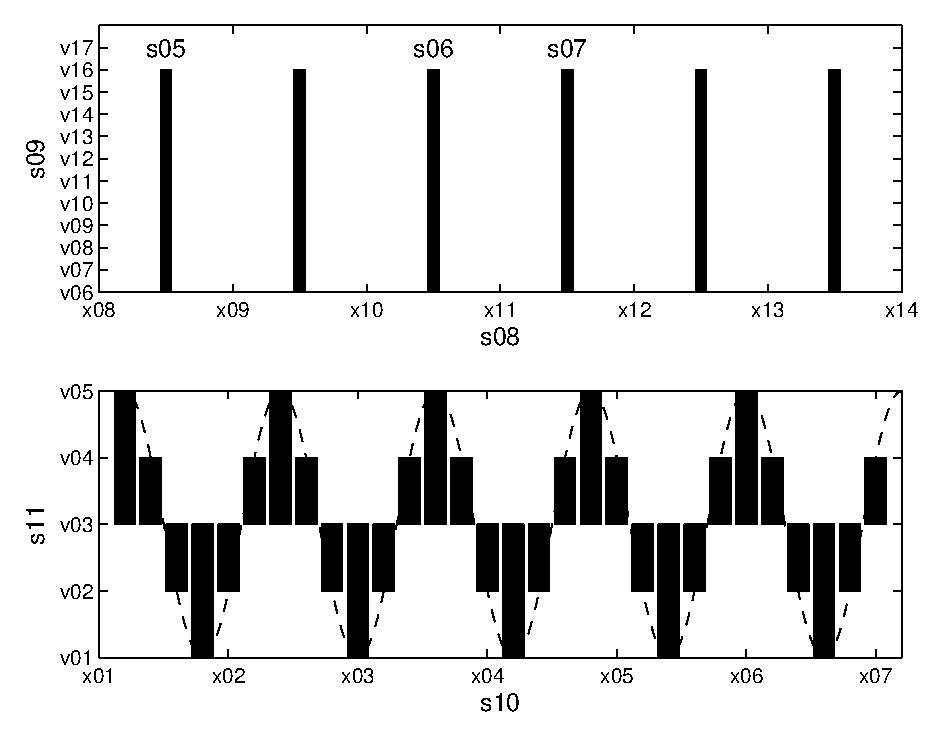
\includegraphics[width=0.9\textwidth]{figs/f_Qs_30_p_5_2.eps}}%
\end{psfrags}%
%
% End f_Qs_30_p_5_2.tex
\end{document}
% See http://www.mathworks.de/matlabcentral/fileexchange/loadFile.do?objectId=4638
% for recent versions of laprint.m.
%
% created by:           LaPrint version 3.16 (13.9.2004)
% created on:           12-Nov-2008 21:50:28
% eps bounding box:     17.5 cm x 13.125 cm
% comment:              
%
\begin{psfrags}%
\psfragscanon%
%
% text strings:
\psfrag{s05}[b][b]{{\tiny $\xi_{5}$}}%
\psfrag{s06}[b][b]{{\tiny $\xi_{25}$}}%
\psfrag{s07}[b][b]{{\tiny $\xi_{35}$}}%
\psfrag{s08}[t][t]{{\tiny $\nu$}}%
\psfrag{s09}[b][b]{{\tiny $\xi_{\nu}$}}%
\psfrag{s10}[t][t]{{\tiny Slot number}}%
\psfrag{s11}[b][b]{{\tiny $F_{slot}/\SI{}{A}$}}%
%
% xticklabels:
\psfrag{x01}[t][t]{{\tiny 0}}%
\psfrag{x02}[t][t]{{\tiny 5}}%
\psfrag{x03}[t][t]{{\tiny 10}}%
\psfrag{x04}[t][t]{{\tiny 15}}%
\psfrag{x05}[t][t]{{\tiny 20}}%
\psfrag{x06}[t][t]{{\tiny 25}}%
\psfrag{x07}[t][t]{{\tiny 30}}%
\psfrag{x08}[t][t]{{\tiny 0}}%
\psfrag{x09}[t][t]{{\tiny 10}}%
\psfrag{x10}[t][t]{{\tiny 20}}%
\psfrag{x11}[t][t]{{\tiny 30}}%
\psfrag{x12}[t][t]{{\tiny 40}}%
\psfrag{x13}[t][t]{{\tiny 50}}%
\psfrag{x14}[t][t]{{\tiny 60}}%
%
% yticklabels:
\psfrag{v01}[r][r]{{\tiny -2}}%
\psfrag{v02}[r][r]{{\tiny -1}}%
\psfrag{v03}[r][r]{{\tiny 0}}%
\psfrag{v04}[r][r]{{\tiny 1}}%
\psfrag{v05}[r][r]{{\tiny 2}}%
\psfrag{v06}[r][r]{{\tiny 0}}%
\psfrag{v07}[r][r]{{\tiny 0.1}}%
\psfrag{v08}[r][r]{{\tiny 0.2}}%
\psfrag{v09}[r][r]{{\tiny 0.3}}%
\psfrag{v10}[r][r]{{\tiny 0.4}}%
\psfrag{v11}[r][r]{{\tiny 0.5}}%
\psfrag{v12}[r][r]{{\tiny 0.6}}%
\psfrag{v13}[r][r]{{\tiny 0.7}}%
\psfrag{v14}[r][r]{{\tiny 0.8}}%
\psfrag{v15}[r][r]{{\tiny 0.9}}%
\psfrag{v16}[r][r]{{\tiny 1}}%
\psfrag{v17}[r][r]{{\tiny 1.1}}%
%
% Figure:

\subfloat[Slot mmf and winding factors\label{fig:f_Qs30_p5_2}]{%
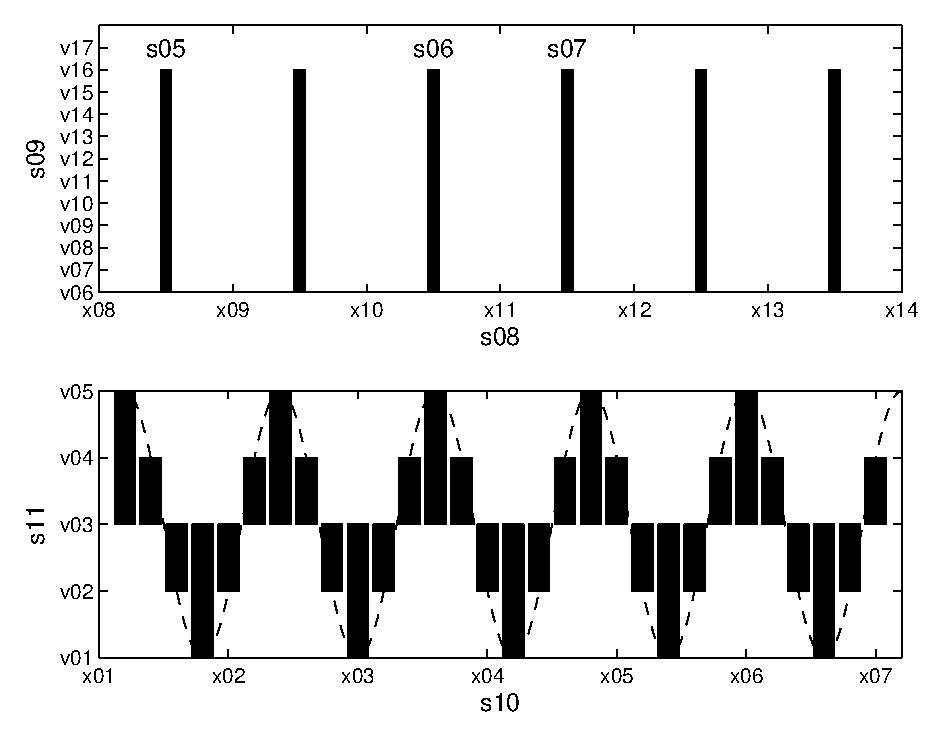
\includegraphics[width=0.9\textwidth]{figs/f_Qs_30_p_5_2.eps}}%
\end{psfrags}%
%
% End f_Qs_30_p_5_2.tex
\end{document}
% See http://www.mathworks.de/matlabcentral/fileexchange/loadFile.do?objectId=4638
% for recent versions of laprint.m.
%
% created by:           LaPrint version 3.16 (13.9.2004)
% created on:           12-Nov-2008 21:50:28
% eps bounding box:     17.5 cm x 13.125 cm
% comment:              
%
\begin{psfrags}%
\psfragscanon%
%
% text strings:
\psfrag{s05}[b][b]{{\tiny $\xi_{5}$}}%
\psfrag{s06}[b][b]{{\tiny $\xi_{25}$}}%
\psfrag{s07}[b][b]{{\tiny $\xi_{35}$}}%
\psfrag{s08}[t][t]{{\tiny $\nu$}}%
\psfrag{s09}[b][b]{{\tiny $\xi_{\nu}$}}%
\psfrag{s10}[t][t]{{\tiny Slot number}}%
\psfrag{s11}[b][b]{{\tiny $F_{slot}/\SI{}{A}$}}%
%
% xticklabels:
\psfrag{x01}[t][t]{{\tiny 0}}%
\psfrag{x02}[t][t]{{\tiny 5}}%
\psfrag{x03}[t][t]{{\tiny 10}}%
\psfrag{x04}[t][t]{{\tiny 15}}%
\psfrag{x05}[t][t]{{\tiny 20}}%
\psfrag{x06}[t][t]{{\tiny 25}}%
\psfrag{x07}[t][t]{{\tiny 30}}%
\psfrag{x08}[t][t]{{\tiny 0}}%
\psfrag{x09}[t][t]{{\tiny 10}}%
\psfrag{x10}[t][t]{{\tiny 20}}%
\psfrag{x11}[t][t]{{\tiny 30}}%
\psfrag{x12}[t][t]{{\tiny 40}}%
\psfrag{x13}[t][t]{{\tiny 50}}%
\psfrag{x14}[t][t]{{\tiny 60}}%
%
% yticklabels:
\psfrag{v01}[r][r]{{\tiny -2}}%
\psfrag{v02}[r][r]{{\tiny -1}}%
\psfrag{v03}[r][r]{{\tiny 0}}%
\psfrag{v04}[r][r]{{\tiny 1}}%
\psfrag{v05}[r][r]{{\tiny 2}}%
\psfrag{v06}[r][r]{{\tiny 0}}%
\psfrag{v07}[r][r]{{\tiny 0.1}}%
\psfrag{v08}[r][r]{{\tiny 0.2}}%
\psfrag{v09}[r][r]{{\tiny 0.3}}%
\psfrag{v10}[r][r]{{\tiny 0.4}}%
\psfrag{v11}[r][r]{{\tiny 0.5}}%
\psfrag{v12}[r][r]{{\tiny 0.6}}%
\psfrag{v13}[r][r]{{\tiny 0.7}}%
\psfrag{v14}[r][r]{{\tiny 0.8}}%
\psfrag{v15}[r][r]{{\tiny 0.9}}%
\psfrag{v16}[r][r]{{\tiny 1}}%
\psfrag{v17}[r][r]{{\tiny 1.1}}%
%
% Figure:

\subfloat[Slot mmf and winding factors\label{fig:f_Qs30_p5_2}]{%
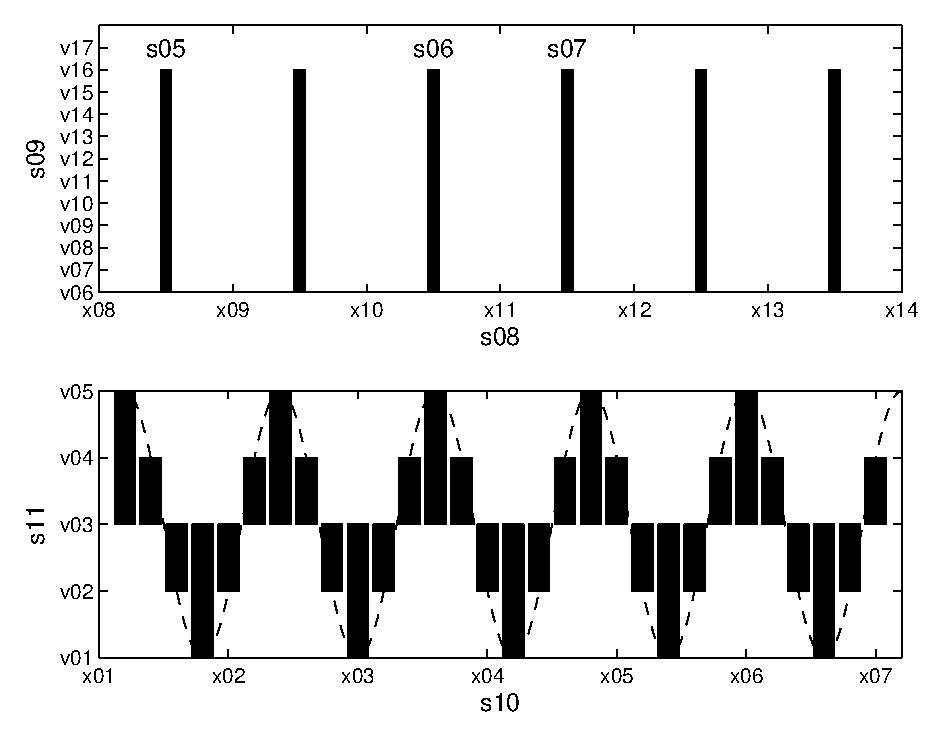
\includegraphics[width=0.9\textwidth]{figs/f_Qs_30_p_5_2.eps}}%
\end{psfrags}%
%
% End f_Qs_30_p_5_2.tex
\end{document}
% See http://www.mathworks.de/matlabcentral/fileexchange/loadFile.do?objectId=4638
% for recent versions of laprint.m.
%
% created by:           LaPrint version 3.16 (13.9.2004)
% created on:           12-Nov-2008 21:50:28
% eps bounding box:     17.5 cm x 13.125 cm
% comment:              
%
\begin{psfrags}%
\psfragscanon%
%
% text strings:
\psfrag{s05}[b][b]{$\xi_{5}$}
\psfrag{s06}[b][b]{$\xi_{25}$}
\psfrag{s07}[b][b]{$\xi_{35}$}
\psfrag{s08}[t][t]{$\nu$}
\psfrag{s09}[b][b]{$\xi_{\nu}$}
\psfrag{s10}[t][t]{Slot number}
\psfrag{s11}[b][b]{$F_{slot}/\SI{}{A}$}
%
% xticklabels:
\psfrag{x01}[t][t]{0}
\psfrag{x02}[t][t]{5}
\psfrag{x03}[t][t]{10}
\psfrag{x04}[t][t]{15}
\psfrag{x05}[t][t]{20}
\psfrag{x06}[t][t]{25}
\psfrag{x07}[t][t]{30}
\psfrag{x08}[t][t]{0}
\psfrag{x09}[t][t]{10}
\psfrag{x10}[t][t]{20}
\psfrag{x11}[t][t]{30}
\psfrag{x12}[t][t]{40}
\psfrag{x13}[t][t]{50}
\psfrag{x14}[t][t]{60}
%
% yticklabels:
\psfrag{v01}[r][r]{-2}
\psfrag{v02}[r][r]{-1}
\psfrag{v03}[r][r]{0}
\psfrag{v04}[r][r]{1}
\psfrag{v05}[r][r]{2}
\psfrag{v06}[r][r]{0}
\psfrag{v07}[r][r]{0.1}
\psfrag{v08}[r][r]{0.2}
\psfrag{v09}[r][r]{0.3}
\psfrag{v10}[r][r]{0.4}
\psfrag{v11}[r][r]{0.5}
\psfrag{v12}[r][r]{0.6}
\psfrag{v13}[r][r]{0.7}
\psfrag{v14}[r][r]{0.8}
\psfrag{v15}[r][r]{0.9}
\psfrag{v16}[r][r]{1}
\psfrag{v17}[r][r]{1.1}
%
% Figure:
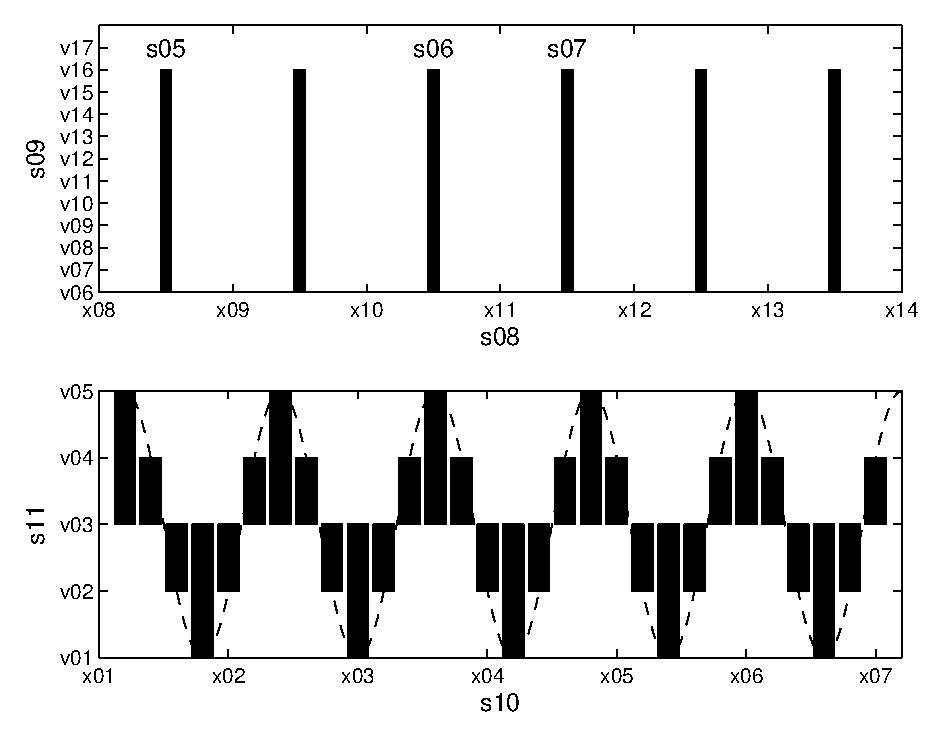
\includegraphics[width=0.47\textwidth]{figs/f_Qs_30_p_5_2.eps}
\end{psfrags}%
%
% End f_Qs_30_p_5_2.tex
